% Pre-ambulo
\documentclass[a4paper, 12pt]{abnt}

\usepackage[brazil]{babel}
\usepackage[T1]{fontenc}
\usepackage[utf8]{inputenc}
\usepackage{dsfont}
\usepackage{amssymb,amsmath}
\usepackage{multirow}
\usepackage[alf]{abntcite}
\usepackage[pdftex]{color, graphicx}
\usepackage{graphicx,graphics}
\usepackage{colortbl}
\usepackage{url}
\usepackage{abnt-alf}
\usepackage{abntcite}
\usepackage{algorithm}
\usepackage{algorithmic}
\usepackage{tabularx}
\usepackage{lipsum}
\usepackage{enumitem}
\usepackage[ampersand]{easylist}
\usepackage{hyperref}
\usepackage{float}
\usepackage{caption}
\usepackage[table,xcdraw]{xcolor}

%\usepackage{alg}

% Redefinicao de instrucoes
\floatname{algorithm}{Algoritmo}
\renewcommand{\algorithmicrequire}{\textbf{Entrada:}}
\renewcommand{\algorithmicensure}{\textbf{Saída:}}
\renewcommand{\algorithmicend}{\textbf{fim}}
\renewcommand{\algorithmicif}{\textbf{se}}
\renewcommand{\algorithmicthen}{\textbf{então}}
\renewcommand{\algorithmicelse}{\textbf{senão}}
\renewcommand{\algorithmicfor}{\textbf{para}}
\renewcommand{\algorithmicforall}{\textbf{para todo}}
\renewcommand{\algorithmicdo}{\textbf{faça}}
\renewcommand{\algorithmicwhile}{\textbf{enquanto}}
\renewcommand{\algorithmicloop}{\textbf{loop}}
\renewcommand{\algorithmicrepeat}{\textbf{repetir}}
\renewcommand{\algorithmicuntil}{\textbf{até que}}
\renewcommand{\algorithmiccomment}[1]{\% #1}


\newcommand{\ignore}[1]{}


\def\twodigits#1{% 
\ifnum#1<10 0\fi 
\number#1}

% Hifenização de palavras feita de forma incorreta pelo LaTeX
\hyphenation{PYTHON ou-tros}

% Inicio do documento
\begin{document}
	
	\frenchspacing
		
	% Capa (arquivo Includes/Capa.tex)
	% Capa
% Proteção externa do trabalho e sobre a qual se imprimem as informações indispensáveis 
% à sua identificação.

% Especificação da capa
\begin{titlepage}
	\begin{center}
		
		% Cabeçalho (não deve ser modificado)
		% Contém o brasão da Universidade, o logotipo do Departamento, além dos dados
		% relacionados à vinculação do aluno (Universidade, Centro, Departamento e Curso)
		\begin{minipage}{2cm}
			\begin{center}
				
\includegraphics[width=1.7cm, height=2.0cm]{Images/Brasao-UFRN.jpg}
			\end{center}
		\end{minipage}
		\begin{minipage}{11cm}
			\begin{center}
				\begin{espacosimples}
					{\small \textsc{Universidade Federal do Rio Grande do Norte}			\\
							  \textsc{Centro de Ciências Exatas e da Terra}						\\
							  \textsc{Departamento de Informática e Matemática Aplicada}	\\
							  \textsc{Bacharelado em Engenharia de Software}}
				\end{espacosimples}
			\end{center}
		\end{minipage}
		\begin{minipage}{2cm}
			\begin{center}
				
\includegraphics[width=1.8cm, height=1.5cm]{Images/Logotipo-DIMAp.jpg}
			\end{center}
		\end{minipage}
			
		\vspace{6cm}
						
		% Título do trabalho
		{\setlength{\baselineskip}%
		{1.3\baselineskip}
		{\LARGE \textbf{Especificação e Desenvolvimento do Sistema de Gestão de Produção Multimídia (Gema) para o Instituto Metrópole Digital}}\par}
			
		\vspace{4cm}
			
		% Nome do aluno (autor)
		{\large \textbf{Wendell Pamplona Barreto}}
						
		\vspace{7cm}
		
		% Local da instituição onde o trabalho deve ser apresentado e ano de entrega do mesmo
		Natal-RN\\Novembro de 2016
	\end{center}
\end{titlepage}

	% Folha de rosto (arquivo Includes/FolhaRosto.tex)
	% Folha de rosto
% Contém os elementos essenciais à identificação do trabalho.

% Título, nome do aluno e respectivo orientador e filiação
\titulo{\Large{Especificação e Desenvolvimento do Sistema de Materiais (SiMate) para o Instituto Metrópole Digital}}
\autor{Wendell Pamplona Barreto}
\orientador[Orientador(a)]{\par Prof. Dr. Marcel Oliveira}
\instituicao
{
	Universidade Federal do Rio Grande do Norte -- UFRN \par 
	Departamento de Informática e Matemática Aplicada -- DIMAp
}
	
% Natureza do trabalho (não deve ser modificada)
\comentario
{
	Proposta de Monografia de Graduação apresentada ao Departamento de Informática e Matemática Aplicada do 
	Centro de Ciências Exatas e da Terra da Universidade Federal do Rio Grande do Norte como
	requisito parcial para a obtenção do grau de bacharel em Engenharia de Software.
}
		
% Local e data
\local{Natal-RN}
\data{Outubro 2015}
	
\folhaderosto	
	
	% Folha de aprovacao (arquivo Includes/FolhaAprovacao.tex)
	% Folha de aprovação
\begin{folhadeaprovacao}
	\setlength{\ABNTsignthickness}{0.4pt}
	\setlength{\ABNTsignwidth}{10cm}
	
	% Informações gerais acerca do trabalho 
	% (nome do autor, título, instituição à qual é submetido e natureza)
	\noindent 
	\textbf{Trabalho de conclusão de curso} sob o título \textit{Especificação e Desenvolvimento do Sistema de Gerência de Materiais (Gema) para o Instituto Metrópole Digital} apresentado por 
	Wendell Pamplona Barreto e aceita pelo Departamento de Informática e Matemática Aplicada do
	Centro de Ciências Exatas e da Terra da Universidade Federal do Rio Grande do Norte,
	sendo aprovada por todos os membros da banca examinadora abaixo especificada:
		
	% Membros da banca examinadora e respectivas filiações
	\assinatura
	{
		Prof. Dr. Marcel Vinícius Medeiros Oliveira\\
		{\small Orientador} 															\\ 
		{\footnotesize
			Departamento de Informática e Matemática Aplicada do Centro de Ciências Exatas e da Terra \\
			Universidade Federal do Rio Grande do Norte
		}
	}
	
	\assinatura
	{
		Prof. Dr. Itamir de Morais Barroca Filho						\\
		%{\small Co-orientador(a), se houver}										\\ 
		{\footnotesize
			Instituto Metrópole Digital \\
			Universidade Federal do Rio Grande do Norte
		}
	}
		
	\assinatura
	{
		Prof. Dr. Jair Cavalcanti Leite					 \\ 
		{\footnotesize
			Departamento de Informática e Matemática Aplicada do Centro de Ciências Exatas e da Terra \\
			Universidade Federal do Rio Grande do Norte
		}
	}
	\vfill
	
	\begin{center}
		Natal-RN, 30 de Novembro de 2016.
	\end{center}
\end{folhadeaprovacao}	
	
	% Dedicatoria (arquivo Includes/Dedicatoria.tex)
	%% Dedicatória

\chapter*{}
\vspace{15cm}
\begin{flushright}
	
	
	\vspace{4cm}


\end{flushright}
	
	% Agradecimentos (arquivo Includes/Agradecimentos.tex)
	%% Agradecimentos

\chapter*{Agradecimentos}



\vspace{4cm}


   
    % Epigrafe (arquivo Includes/Epigrafe.tex)
	% Epígrafe (citação seguida de indicação de autoria)

\chapter*{}

\vspace{4cm}


\vspace{11cm}
\begin{flushright}
	\textit
	{
		If you want work well done, select a busy man‚ the other kind has no time.
	}\medskip\\ 
	Elbert Hubbard
\end{flushright}
	
	% Resumo em língua vernacula (arquivo Includes/Resumo.tex)
	% Resumo em língua vernácula
\begin{center}
	{\Large{\textbf{Especificação e Desenvolvimento do Sistema de Gerência de Materiais (Gema) para o Instituto Metrópole Digital}}}
\end{center}

\vspace{1cm}

\begin{flushright}
	Autor: Wendell Pamplona Barreto\\
	Orientador: Prof. Dr. Marcel Vinícius Medeiros Oliveira
\end{flushright}

\vspace{1cm}

\begin{center}
	\Large{\textsc{\textbf{Resumo}}}
\end{center}

\noindent A maneira como as organizações e instituições dependem dos sistemas de informações pra alavancar seus desempenhos e se sobressair no mercado é notável. Diante dos estudos da tecnologia da informação, soluções são desenvolvidas com foco em optimizar e aprimorar os processos. Perante essas necessidades, este trabalho propõe uma solução de software que busca optimizar o processo de criação de materiais no setor de produção de materiais do Instituto Metrópole Digital, unidade suplementar da Universidade Federal do Rio Grande do Norte. Através dessa proposta, o estudo de caso será realizado para levantar os requisitos necessários para o desenvolvimento, assim como validá-los com os envolvidos, garantindo assim que o modelo de software proposto atenda a demanda dos usuários. 

\noindent\textit{Palavras-chave}: sistema de informação, desenvolvimento, processos, materiais.
	
	% Abstract, resumo em língua estrangeira (arquivo Include/Abstract.tex)
	% Resumo em língua estrangeira (em inglês Abstract, em espanhol Resumen, em francês Résumé)
\begin{center}
	{\Large{\textbf{Specification and Development of Materials System (SiMate) for the Digital Metropolis Institute}}}
\end{center}

\vspace{1cm}

\begin{flushright}
	Author: Wendell Pamplona Barreto\\
	Advisor: Prof. Dr. Marcel Oliveira
\end{flushright}

\vspace{1cm}

\begin{center}
	\Large{\textsc{\textbf{Abstract}}}
\end{center}

\noindent The way that the organizations and institutions depend on information systems to leverage your performance and excel in the market is remarkable. Given the information technology studies, solutions are developed with a focus on optimizing and improving processes. And given these needs, this paper proposes a software solution that seeks to optimize the process of creating materials in the Digital Metropolis Institute materials production sector, supplementary unit of the Federal University of Rio Grande do Norte. Through this proposal, the case study will be conducted to raise the requirements for the development, and validate them with the stakeholders, thereby ensuring that the proposed software model meets the demands of users.

\noindent\textit{Keywords}: information system, development, process, materials.
	
	% Lista de figuras mas so caso tiver figuras
	\listoffigures

	% Lista de tabelas mas so caso tiver tabelas
	\listoftables
	
	% Lista de abreviaturas e siglas mas so caso tiver siglas
	%\listadeabreviaturas
	
	% Lista de símbolos mas so caso tiver simbolos especiais
	%\listadesimbolos
	
	% Lista de algoritmos (se houver)
	% Devem ser incluídos os pacotes algorithm e algorithmic
	% \listofalgorithms
	
	% Sumário
	\sumario

	% Parte central do trabalho, englobando os capítulos que constituem o mesmo
	% Os referidos capítulos devem ser organizados dentro do diretório "Capítulos"

	% Capitulo 1: Introdução (arquivo Includes/Introducao.tex)
	% Introdução
\chapter{Introdução}

Este é o capítulo introdutório da monografia e está dividido em cinco seções. A primeira trata de contextualizar o estudo. A segunda trás a situação problema encontrada no contexto informado. Depois disso, são mostradas as possíveis soluções existentes e apresentada a proposta do estudo. Por fim, são expostos os objetivos do trabalho, os métodos e técnicas aplicadas e a motivação encontrada.

\section{Contextualização}

Como Unidade Suplementar da Universidade Federal do Rio Grande do Norte (UFRN), o Instituto Metrópole Digital (IMD) atua na formação de jovens e adultos de nível técnico, superior e pós-graduação. Suas ações integram a inclusão social e digital de estudantes do ensino básico à pós-graduação, a realização de pesquisa e inovação tecnológica e o incentivo à cultura do empreendedorismo.

Hoje o IMD encontra-se particionado em diversos setores, cada qual com seu objetivo e metodologia. Entre estes setores, há o setor de materiais, responsável pela produção de todo o material disponibilizado pelo instituto e principal interessado no desenvolvimento deste trabalho. 

Dentro do setor de materiais é possível extrair todos os fluxos que contemplam a criação de um material e, na figura a seguir, é possível entender como um dos principais fluxos funciona. \\

\vspace{5mm}
\begin{minipage}[c]{\textwidth}
    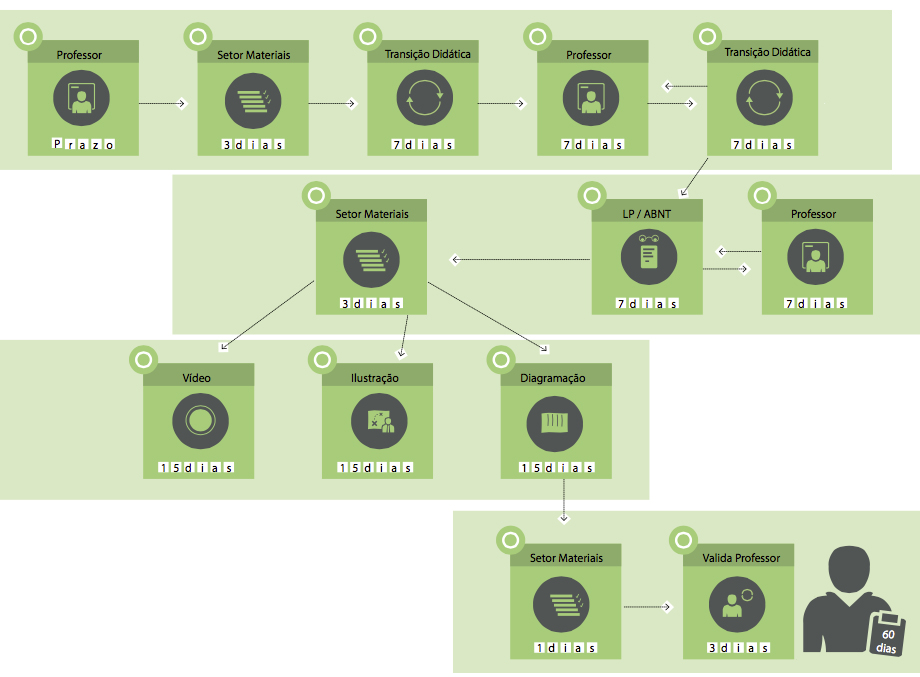
\includegraphics[width=14cm]{Imagens/FluxoMateriaisNovos.jpg}
    \captionof{figure}{Fluxo de Criação de Materiais Didáticos}
    \label{fig:fluxo_materiais_novos}
\end{minipage}
\vspace{5mm}

O fluxo da \hyperref[fig:fluxo_materiais_novos]{Figura \ref{fig:fluxo_materiais_novos}} é iniciado com o envio do arquivo pelo professor para o setor de materiais, onde será feita uma primeira análise do conteúdo do material e será repassado para a equipe pedagógica responsável pela transição didática. O material então fica alternando de etapa entre o professor e a equipe pedagógica até que a última determine a conformidade do conteúdo. Neste momento, a equipe de língua portuguesa e normas ABNT recebe o arquivo e se responsabiliza por executar revisão e melhorias juntamente com o professor, o setor de materiais recebe o resultado e, de acordo com as necessidades, solicita criação de material de vídeo, ilustração e, por último, diagramação. No momento que a equipe de diagramação termina seu trabalho, o arquivo volta ao setor de materiais para que seja feita uma nova verificação nos resultados obtidos e solicitar aprovação ao professor que iniciou o processo.

No fluxo descrito, vários papéis/equipes foram citados, cada um desses é representado na \hyperref[fig:fluxo_materiais_novos]{Figura \ref{fig:fluxo_materiais_novos}} por um bloco verde escuro e destaca um envolvido no processo, alguns deles sendo subsetores do setor de materiais e outros externos a esse. Na tabela abaixo é possível entender os seus papéis.

\begin{center}
    \begin{tabularx}{\textwidth}{ |X|X| }
    \hline
    \multicolumn{2}{|c|}{Definição de envolvidos e papéis} \\
    \hline
    Nome & Papel \\ \hline
    Professor & Elabora o material de aula/prova na sua versão inicial e participa do fluxo realizando melhorias e correções. \\ \hline
    Setor de Materiais & O setor de materiais é principalmente responável por auditar o processo de criação do material. Ele garante a execução dos passos do fluxo, o cumprimento dos prazos e a conformidade com as necessidades. \\ \hline
    Transição Didática & Na transição didática há a formatação textual de acordo com as necessidades pedagógicas da instituição.  \\ \hline
    LP / ABNT & Garante que as normas ortográficas e técnicas do conteúdo do material estejam intactas. \\ \hline
    Vídeo & Realiza criação, gravação e edição dos vídeos necessários para preencher o material didático. \\ \hline
   	Ilustração & Responsável por toda a parte gráfica/artística dos materiais. \\ \hline
   	Diagramação & Define a organização final do material para a publicação. \\ \hline
    \end{tabularx}
\end{center}

Cada processo de criação de material passa por um fluxo dinâmico que envolve um ou mais dos envolvidos descritos acima. Ao entrar num fluxo, o produto segue passando por produções e revisões até se tornar completo e satisfatório para ser distribuído ao público. Público esse que pode ser desde uma campanha tecnológica até os alunos da Educação à Distância (EAD).

\section{Situação Problema}

Os passos quem compõem o fluxo existem com intuito de gerar resultados. Esses resultados representam um produto, mais especificamente um tipo de material que, por sua vez, possui valor para o instituto. 

Tomando como exemplo o fluxo de materiais didáticos novos para as turmas do EAD (ver Figura \ref{fig:fluxo_materiais_novos}), na prática, os passos executados acontecem da seguinte maneira:

\begin{enumerate}
  \item Atráves de correio eletrônico, o professor envia o material com as aulas ao setor de materiais;
  \item Ao receber o arquivo, o setor de materiais cria uma planilha com o estado do material, valida os documentos e passa para a equipe pedagógica;
  \item A equipe de pedagógica executa a revisão textual e reenvia para o professor realizar os ajustes necessários. Esse subprocesso se repete até que a equipe determine que o material está totalmente de acordo com as necessidades percebidas. Ao final, o material é enviado para a revisão LP e ABNT;
  \item A revisão de língua portuguesa e de normas ABNT atua sobre o material recebido trocando emails com o professor até que os textos estejam em conformidade com as normas ortográficas e técnicas.
  \item O resultado do passo anterior deve ser encaminhado para o setor de materiais que atualiza o estado do material na planilha e gerencia os próximos passos. Aqui o setor precisa determinar os elementos de audiovisual que são necessários para completar o material, essas necessidades representas solicitações para a equipe de vídeo, ilustração e, por último, diagramação. 
  \item Ao passo que a equipe de diagramação finaliza seu trabalho, há uma última verificação feita pelo setor de materiais e então é todo o resultado retorna ao professor para a validação final.
\end{enumerate}

Como percebido, cada passagem de etapa do fluxo é feita através de troca de emails e o setor de materiais utiliza de planilhas para gerenciar as versões do material. Uma equipe envia o material atual em anexo para a outra e, no corpo da mensagem, o direcionamento do que fazer e o prazo estipulado, ao final do processo, vários emails foram trocados e há um produto final totalmente validado e pronto pra ser entregue aos alunos.

Na realidade, a forma que o processo descrito é executado possui diversos pontos de falha. O setor de materiais, que é responsável pela criação do material, tem o conhecimento prejudicado sobre o estado do material nas etapas das quais outras equipes são responsáveis. A ferramenta utilizada para o envio também pode facilitar a perda de prazos e até mesmo de qualidade, visto que emails não propriamente enviados ou até mesmo a não percepção do conteúdo que chega na caixa postal da equipe responsável pode acarretar em diminuição do tempo hábil para concretização do trabalho.

A tarefa contínua de verificação do recebimento do material, a necessidade de auditar o processo através de planilhas e outras ferramentas a parte dificultam a saída do material como o processo teoriza. 

% Através da modelagem dos processos, das questões aplicadas e entrevistas semiestruturadas com membros do setor, foi possível identificar as deficiências nos processos produtivos do setor de materiais, para assim, posteriormente, definir todos os requisitos necessários ao sistema de modo a suprir todas as necessidades levantadas.
% A maior deficiência, e a justificativa principal deste trabalho, são as múltiplas ferramentas utilizadas para solicitação e acompanhamento de demanda, visto que desencadeia outros problemas que afetam diretamente o ciclo de trabalho. Os solicitantes são oriundos dos outros setores do instituto. Desde diretores, coordenadores, passando por gerentes, professores e assessores. Como foi introduzido na análise da modelagem dos processos, o relacionamento de alguns solicitantes com a equipe, faz com que eles realizem pedidos informalmente, sem registros de briefing ou análise realista de prazo de execução. A falta de registro impossibilita o responsável pela execução do pedido de acessar as informações, sendo necessário contato
% paralelo com o solicitante, ocasionando possíveis desencontros, lead time maior que o necessário e dificuldade na geração de relatórios operacionais.
% Sobre a geração dos relatórios, este possui outro problema evidenciado na modelagem dos processos e em entrevistas realizadas com os responsáveis pelo gerenciamento do setor. Além de precisar cruzar as informações de diversas fontes manualmente para obtenção de um relatório mais completo, observou-se também a falta de indicadores de desempenho das atividades. Uma tentativa de suprir essa necessidade através de algumas planilhas desenvolvidas no Microsoft Excel7 foi iniciada, no entanto, devido à resistência na utilização das mesmas por parte da equipe, (pela inserção de uma nova ferramenta que precisaria ser administrada, aumentando uma lista, consideravelmente já extensa, de instrumentos de trabalho a serem utilizados.), a ideia não chegou a ser colocada em prática.
% Para definir datas importantes, como entrega de demanda, reuniões, gravação de mídia, não existe um sistema padrão. São utilizados Google Calendar8, Trello, lembretes, etc. Por este motivo, houve registro de divergência de datas, perda de prazos, atrasos, entre outros.
% O fato de não ter os processos modelados e bem definidos para toda a equipe, impossibilita a identificação do percurso de trabalho. A “obscuridade” da produção, faz com que, por exemplo, a equipe “C” não saiba se a etapa está na equipe “B” ou na equipe “A”, tirando o controle necessário para o bom andamento.
% A espera por feedback (e ainda pelos vários meios de informação, não saber ao certo de qual fonte receber) é um problema sofrido principalmente pela equipe de ilustração/diagramação. Visto que eles criam um produto, é necessário o retorno do solicitante para saber se está de acordo com as especificações desejadas. Muitas vezes esse retorno vem depois de muita espera, pedindo alterações urgentes quando a equipe já está sem tempo hábil para atender aos pedidos.

\section{Estado da Arte}

Sob o dever de executar o processo de produção dos materiais, o setor de materiais criou um mecanismo próprio que supre as necessidades e se mostra primordial para o estudo que foi realizado. É com base nesse mecanismo que podemos visualizar quais ferramentas poderiam ser agregadas com o objetivo de automatizar alguns passos e dar suporte no gerenciamento dos fluxos afim de aumentar a qualidade do produto final. Algumas dessas ferramentas foram analisados e suas possíveis formas de atuação serão descritas a seguir.

\subsection{Redmine}

O Redmine é um gerenciador de projeto flexível para Web. Escrito usando Ruby on Rails e disponibilizado sob licença GPL, pode ser configurado para rodar em varias plataformas e suporta diversos bancos de dados. (MOURA; NASCIMENTO, 2010)

Como um gerenciador de projetos baseado na web, o Redmine possui ferramentas de acompanhamento de atividades que permite a atribuição de tarefas para usuários e equipes, o que se mostra bastante razoável no ponto de vista da necessidade principal do setor de materiais. 

Ao pensar no Redmine como uma ferramenta auxiliadora do processo em questão, percebe-se que, através de pequenas adaptações, é possível gerenciar a criação de materiais usando a abordagem de que cada etapa do fluxo seria representado por uma atividade. O setor de materiais seria responsável por criar as atividades e atribuir a cada envolvido responsável e, ao final de cada etapa, executaria o trabalho de transição de atividade para o próximo envolvido até que o material estivesse pronto.

Através da adaptação do processo pra ser usado dentro da ferramenta, é possível entender que essa se mostra interessante mas possui também suas limitações. Ao passo que precisa-se desvincular parte do trabalho de gerenciamento que é feito pelo setor de materiais, ao usar o Redmine, o setor ainda teria que estar intervindo a cada final de etapa e fazendo reatribuições ao longo do fluxo.

\section{Proposta}

Como proposta do estudo feito, surge o desenvolvimento do Sistema de Materiais - SiMAte. Um produto feito de dentro do instituto e modelado juntamente com todos os usuários e demais envolvidos no processo de criação de materiais.

O SiMate tem somo principal atrativo o fato de ser feito totalmente sob medida para solucionar os problemas encontrados no mecanismo atual de produção. A ferramenta aqui apresentada trás consigo todas as funcionalidades chave que o método usado oferece, juntamente com as soluções que outras ferramentas oferecem e melhorias que os usuários poderão perceber ao longo do tempo. Tudo isso unificado em um sistema totalmente extensível e proprietário.

Algumas das necessidades de mais importância levantados na fase de elicitação de requisitos são o versionamento de alteração do material no processo de criação, a definição de papéis para as equipes, a geração de relatórios, a auditoria do fluxo produtivo - o que permite que todos saibam exatamente a etapa atual que a atividade se encontra, o calendário de deadlines, sistema de notificações, definição de prioridades dos produtos e registro de alterações.

Todas esses requisitos serão melhor contextualizados, conceituados e exemplificados no decorrer do estudo.

\section{Organização do trabalho}

\subsection{Objetivos}

Os objetivos desse trabalho são descrever em detalhes o processo de criação de materiais pelo setor de materiais do IMD, encontrar e interpretar a situação problema, definir formas de operação mais eficientes, projetar um mecanismo de software que atenda as novas definições, desenvolver e experimentar a solução proposta. Além disso, o resultado aqui obtido deve não só documentar o projeto, mas também servir de base para a evolução e manutenção do sistema pela equipe responsável.

\subsection{Metodologia}

Como um dos objetivos principais desse trabalho é descrever um processo, adiciona-se a esta pesquisa o teor descritivo. De acordo com Selltiz et al. (1965), a pesquisa descritiva busca descrever um fenômeno ou situação em detalhe, especialmente o que está ocorrendo, permitindo abranger, com exatidão, as características de um indivíduo, uma situação, ou um grupo, bem como desvendar a relação entre os eventos. 

E, ao passo que o estudo feito contempla a análise, teorização de novas formas de execução, projeto de um mecanismo com base nas teorias, desenvolvimento e experimento, pode-se caracterizar essa pesquisa explicativa-experimental.

Entendido a metodologia quanto aos objetivos, nas próximas seções serão explanados os procedimentos utilizados no estudo e como a abordagem do problema foi feita.

\subsubsection{Procedimentos}

Os procedimentos utilizados para entendimento do processo como um todo foram, inicialmente, observação direta da execução do fluxo de criação de materiais. Posteriormente, o levantamento de requisitos foi feito e validado com o setor.

As técnicas utilizadas para levantamento de requisitos se caracterizam como: a) compreensão do domínio, onde o responsável pelo estudo desenvolve o entendimento a partir do contato com o ambiente da aplicação; b) coleta de requisitos, processo em que o analista descobre os requisitos partindo da compreensão do domínio; c) classificação e organização, essa atividade contempla a divisão dos requisitos em grupos de afinidades; d) definição de prioridades, aqui os envolvidos são consultados para que haja a determinação dos requisitos mais importantes; e) verificação e resolução de conflitos, neste último passo os requisitos são verificados para garantir a completude, consistência e se estão em concordância com os envolvidos.

Dados os requisitos, a especificação dos principais é feita através do detalhamento dos cenários de interação entre os usuários e o sistema, atividade também chamada de expansão de casos de uso. Essa expansão busca trazer clareza do fluxo para que todos os eventuais leitores possam entendê-lo de igual forma.

\subsubsection{Abordagem da Situação Problema}

Conforme já exposto, a situação problema é abordada com o propósito de teorizar sobre formas mais eficientes de execução do processo, documentá-las e desenvolver um mecanismo de software que atenda essas determinações.

\subsection{Motivação}

Todos os dias novos produtos surgem no mercado tecnológico com o objetivo de solucionar algum problema do cotidiano de empresas e instituições. O SiMate, como sistema de informação, é proposto com o intuito lapidar processos diretamente relacionados com a criação de materiais didáticos, interesse cuja preocupação deve ser notória, pois, à medida que o produto da instituição é o ensino, a qualificação dos seus alunos deve ser seu carro chefe.

No Instituto Metrópole Digital, assim como nos demais institutos de ensino, os benefícios que os recursos tecnológicos presentes fornecem precisam ser melhor aproveitados e, para isso, a percepção do poder da tecnologia da informação e a adesão ao novo devem ser praticados. 

Este trabalho nada mais é do que e prática desses comportamentos. O sistema aqui proposto é um modelo totalmente baseado nas necessidades do setor e que proporcionará o domínio dos processos produtivos e o aumento de performance do trabalho executado.

	
	% Capitulo 2: Segundo capítulo (arquivo Includes/SiMate.tex)
	%% SiMate

\chapter{SiMate: Sistema de Materiais}

\section{Elicitação de Requisitos}

Tomando como base o contexto do sistema, os requisitos foram elicitados e, nesta seção, estão divididos em regras de negócios, requisitos funcionais e requisitos não funcionais.

Para facilitar o entendimento e evitar a repetição desnecessária, a sigla CRUD (acrónimo de Create, Read, Update e Delete na língua Inglesa) será usada como representação das ações de criação, visualização, edição e exclusão do modelo associado.

\subsection{Regras de Negócio} \label{subsec:regras_de_negocio}

Regras de negócio declaram e refletem as regras do produto, definindo assim as instruções de como o sistema irá atingir o seu objetivo obedecendo a políticas internas, o processo definido e as determinações básicas de conduta. 

Nesta subseção serão definidas as restrições, validações, comportamentos, exceções e os demais elementos que compõem o conjunto de instruções que o sistema a ser desenvolvido deve contemplar..

\begin{enumerate}[label=\textbf{RN\protect\twodigits{\theenumi}}, leftmargin=2cm]
	\item \label{rn:administrador} Todos os usuários que possuírem o papel de Administrador devem ter completo acesso a todas as funcionalidades do sistema (ver \hyperref[subsec:requisitos_funcionais]{Requisitos Funcionais}). \\
		\textbf{Prioridade:} Alta \\
		\textbf{Depende de:} Nenhum

	\item \label{rn:artefato_na_etapa} Após entrar em um fluxo, o material de aula ou prova (artefato) só pode participar de uma etapa por vez. Estando em uma etapa, somente os usuários que possuem o papel responsável pela etapa em questão podem agir sobre o artefato, fazendo alterações, avaliações e o repassando para uma das próximas etapas disponíveis. Essa regra não vale para usuários com papel de administrador (ver \hyperref[rn:administrador]{\ref{rn:administrador}}). \\
		\textbf{Prioridade:} Média \\
		\textbf{Depende de:} \hyperref[rn:administrador]{\ref{rn:administrador}}

	\item \label{rn:etapa_inicial_e_final_do_fluxo} O fluxo do material pode ser representado por um grafo de arestas bidirecionas. Dessa forma, não há definição do vértice (etapa) inicial e final, logo é necessário que o fluxo guarde explicitamente o nome dessas duas etapas. \\
		\textbf{Prioridade:} Alta \\
		\textbf{Depende de:} Nenhum

\end{enumerate}

\subsection{Requisitos Funcionais} \label{subsec:requisitos_funcionais}
		
\begin{enumerate}[label=\textbf{RF\protect\twodigits{\theenumi}}, leftmargin=2cm]

	\item \label{rf:papeis} O sistema deve permitir o gerenciamento (CRUD) dos papéis. Cada papel representa uma função que pode ser exercida por um ou mais usuários. As determinações dessas funções podem ser entendidas na subseção \hyperref[subsec:regras_de_negocio]{Regras de Negócio} \\
		\textbf{Prioridade:} Alta \\
		\textbf{Depende de:} \hyperref[rn:administrador]{\ref{rn:administrador}}

	\item \label{rf:usuarios} O sistema deve permitir, além das ações de CRUD, o login e logout dos usuários. \\
		\textbf{Prioridade:} Alta \\
		\textbf{Depende de:} Nenhum

	\item \label{rf:etapas} O sistema deve permitir o gerenciamento (CRUD) das etapas. A etapa representa o estado em que um material de aula ou prova (artefato) pode estar dentro de um fluxo. Se um material de aula é enviado de um professor para a revisão didática, por exemplo, podemos dizer que o artefato em questão está na etapa de transição didática e que os responsáveis pela revisão são os usuários que possuem o papel de equipe de transição didática.  \\
		\textbf{Prioridade:} Alta \\
		\textbf{Depende de:} \hyperref[rn:artefato_na_etapa]{\ref{rn:artefato_na_etapa}}

	\item \label{rf:fluxos} O sistema deve permitir o gerenciamento (CRUD) dos fluxos. Para melhor entendimento, pode-se pensar no fluxo como um grafo de arestas bidirecionais, onde cada vértice é uma etapa e as arestas são possibilidades de transição das etapas do material. \\ 
	Por exemplo, estando um material de aula na etapa de transição didática (vértice) ela pode seguir para a correção do professor (aresta ligando etapa de transição didática e etapa de correção do professor) ou pode ir para a revisão LP/ABNT (aresta ligando etapa de transição didática à etapa de revisão LP/ABNT). Como a representação de grafo aqui definida não sugere etapa inicial e final, o fluxo deve guardar explicitamente a determinação dessas duas etapas (ver \hyperref[rn:etapa_inicial_e_final_do_fluxo]{\ref{rn:etapa_inicial_e_final_do_fluxo}}). \\
		\textbf{Prioridade:} Alta \\
		\textbf{Depende de:} \hyperref[rf:etapas]{\ref{rf:etapas}}

	\item \label{rf:artefatos} O sistema deve permitir o gerenciamento (CRUD) de artefatos. O artefato pode assumir um dos seguintes tipos: aula ou prova. Ele tem uma data de entrega e pertence a uma oferta. Além disso, cada artefato possui n versões, sendo n definido pelo número de etapas que o artefato passou dentro do fluxo da sua oferta. Cada versão é caracterizada por ter autor, data de criação, arquivo e mensagem. \\
		\textbf{Prioridade:} Alta \\
		\textbf{Depende de:} \hyperref[rf:ofertas]{\ref{rf:ofertas}} e \hyperref[rf:fluxos]{\ref{rf:fluxos}}
				
	\item \label{rf:modulos} O sistema deve permitir o gerenciamento (CRUD) dos módulos. Cada módulo representa um espaço de tempo de um determinado ano com datas de início e fim bem definidas. Os módulos participam de um semestre, ou seja, cada módulo possui associação com um semestre do ano letivo. \\
		\textbf{Prioridade:} Alta \\
		\textbf{Depende de:} Nenhum

	\item \label{rf:disciplinas} O sistema deve permitir o gerenciamento (CRUD) de disciplinas. Disciplinas representam áreas do conhecimento que serão posteriormente usadas para criar as ofertas. \\
		\textbf{Prioridade:} Alta \\
		\textbf{Depende de:} Nenhum
		
	\item \label{rf:ofertas} O sistema deve permitir o gerenciamento (CRUD) de ofertas. Cada oferta designa, de fato, o conjunto de aulas e provas (artefatos) de uma área de conhecimento (disciplina) que acontecem em um determinado período de um semestre (módulo). \\
		\textbf{Prioridade:} Alta \\
		\textbf{Depende de:} \hyperref[rf:modulos]{\ref{rf:modulos}}, \hyperref[rf:disciplinas]{\ref{rf:disciplinas}}, \hyperref[rf:fluxos]{\ref{rf:fluxos}} e \hyperref[rf:artefatos]{\ref{rf:artefatos}}
		
	\item \label{rf:fluxo} O sistema deve permitir a criação dos materiais. Essa criação pode ser definida como um conjunto de passos que adicionam, validam e corrigem o material, permitindo assim que ele esteja pronto para ser usado ao final do fluxo. \\
	O passo introdutório do processo de elaboração da aula/prova deve ser dado pelo usuário responsável pela etapa inicial, permitindo assim que as outras etapas aconteçam até que o material chegue a etapa conclusiva. \\	
	\textbf{Prioridade:} Alta \\
	\textbf{Depende de:} \hyperref[rn:artefato_na_etapa]{\ref{rn:artefato_na_etapa}}, \hyperref[rn:etapa_inicial_e_final_do_fluxo]{\ref{rn:etapa_inicial_e_final_do_fluxo}}, \hyperref[rf:papeis]{\ref{rf:papeis}}, \hyperref[rf:usuarios]{\ref{rf:usuarios}}, \hyperref[rf:etapas]{\ref{rf:etapas}}, \hyperref[rf:fluxos]{\ref{rf:fluxos}}, \hyperref[rf:artefatos]{\ref{rf:artefatos}}, \hyperref[rf:modulos]{\ref{rf:modulos}}, \hyperref[rf:disciplinas]{\ref{rf:disciplinas}} e \hyperref[rf:ofertas]{\ref{rf:ofertas}}
	
\end{enumerate}

\subsection{Requisitos Não-Funcionais}

\begin{enumerate}[label=\textbf{RNF\protect\twodigits{\theenumi}}, leftmargin=2cm]

	\item \label{rf:papeis} O sistema deve estar disponível 24 horas/dia e 7 dias/semana, a fim de garantir que as metas estabelecidas para criação dos materiais não sejam quebradas por indisponibilidade da aplicação. \\
		\textbf{Categoria:} Disponibilidade e Confiabilidade \\
		\textbf{Escopo:} Sistema \\
		\textbf{Prioridade:} Alta \\
		\textbf{Depende de:} Nenhum

	\item \label{rf:papeis} O sistema deve lidar com os vários níveis de acesso dos usuários restringindo a interação com os conteúdos a eles associados. \\
		\textbf{Categoria:} Segurança de Acesso \\
		\textbf{Escopo:} Funcionalidade \\
		\textbf{Prioridade:} Alta \\
		\textbf{Depende de:} Nenhum

	\item \label{rf:papeis} O sistema deve trazer uma interface amigável, simples, rápida e eficiente. \\
		\textbf{Categoria:} Usabilidade, Atratividade e Desempenho \\
		\textbf{Escopo:} Sistema \\
		\textbf{Prioridade:} Alta \\
		\textbf{Depende de:} Nenhum

	\item \label{rf:papeis} Para garantir a fácil manutenção pela equipe a qual será entregue o sistema após o desenvolvimento, esse deve ser implementado utilizando a linguagem de programação JAVA. \\
		\textbf{Categoria:} Implementação \\
		\textbf{Escopo:} Sistema \\
		\textbf{Prioridade:} Alta \\
		\textbf{Depende de:} Nenhum

\end{enumerate}

\section{Especificação de Casos de Uso}

Nesta seção serão especificados as unidades funcionais que representam as necessidades principais do sistema. No primeiro tópico, os atores participantes dessas funcionalidades serão conceituados e, após isso, será feito o detalhamento dos casos de uso.

\subsection{Atores}

\subsubsection{Administrador}

O ator Administrador representa a pessoa que tem poder total sobre o sistema. Nenhuma funcionalidade é restringida a esse tipo de usuário.

\subsubsection{Setor de Materiais}

No sistema, o usuário possuidor do papel de Setor de Materiais é responsável principalmente por gerir a execução do fluxo, permitindo assim auditoria e intervenção no processo.

\subsubsection{Membro}

O ator Membro existe para representar usuários como o professor e os membros das demais equipes no sistema. O principal objetivo desse tipo de usuário é participar do fluxo de materiais contribuindo para que o material seja desenvolvido.

\subsection{Casos de Uso}
     
\begin{enumerate}[label=\textbf{UC01}, leftmargin=2cm]
	\item \textbf{Criar Etapa} \\
	A etapa representa um possível passo em qualquer fluxo, dessa forma, cada etapa pode participar de diversos fluxos ao mesmo tempo, sendo a ela atribuído somente nome, responsáveis e descrição. \\
	\begin{minipage}[c]{10cm}
	    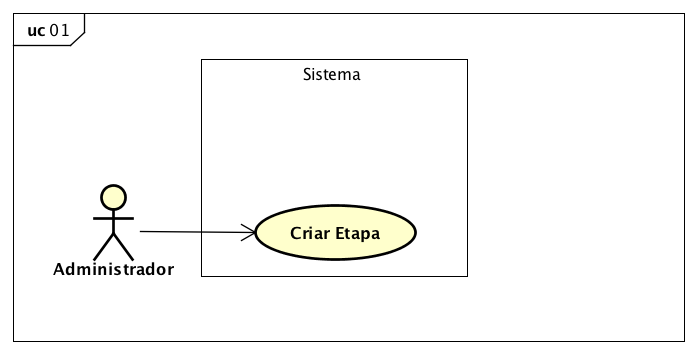
\includegraphics[width=10cm]{Imagens/UC_CriarEtapa.png}
	    \captionof{figure}{Diagrama do Caso de Uso Criar Etapa}
		\label{fig:uc_criar_fluxo}
	\end{minipage} \\

	\begin{enumerate}[label=, leftmargin=0cm]
		\item \textbf{Atores} \\
		Administrador
		\item \textbf{Precondições}
			\begin{enumerate}[label=\arabic*.]
				\item Usuário estar logado no sistema.
			\end{enumerate}
		\item \textbf{Fluxo Básico}
			\begin{enumerate}[label=\arabic*.]
				\item Usuário solicita o formulário de criação de etapa.
				\item O sistema exibe formulário onde o usuário deve preencher o nome da etapa, os papéis pela execução da etapa e uma descrição.
				\item Usuário preenche formulário.
				\item O sistema valida os dados e informa que o fluxo com salvo com sucesso.
			\end{enumerate}
		\item \textbf{Pós-condições}
			\begin{enumerate}[label=\arabic*.]
				\item Uma nova etapa foi criada e pode ser visualizado, editado, excluído ter passos do fluxo associados a ela.
			\end{enumerate}
	\end{enumerate}
	 
\end{enumerate}

\begin{enumerate}[label=\textbf{U02}, leftmargin=2cm]
	\item \textbf{Criar Fluxo} \\
	Este caso de de uso detalha a elaboração do fluxo e suas etapas. No sistema, um fluxo criado representa o passo-a-passo para a criação dos materiais associados. \\
	\begin{minipage}[c]{10cm}
	    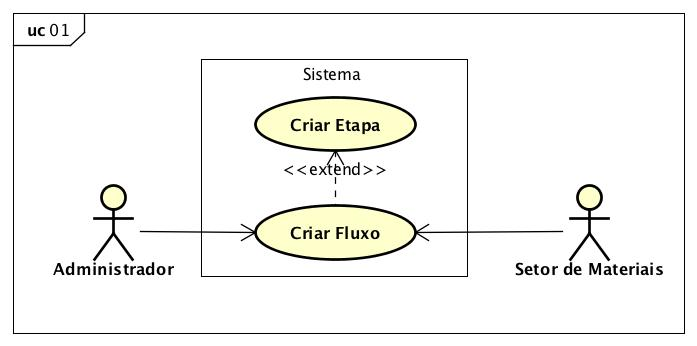
\includegraphics[width=10cm]{Imagens/UC_CriarFluxo.jpg}
	    \captionof{figure}{Diagrama do Caso de Uso Criar Fluxo}
		\label{fig:uc_criar_fluxo}
	\end{minipage} \\

	\begin{enumerate}[label=, leftmargin=0cm]
		\item \textbf{Atores} \\
		Administrador e Setor de Materiais
		\item \textbf{Precondições}
			\begin{enumerate}[label=\arabic*.]
				\item Usuário estar logado no sistema.
			\end{enumerate}
		\item \textbf{Fluxo Básico}
			\begin{enumerate}[label=\arabic*.]
				\item Usuário solicita o formulário de criação de fluxo.
				\item O sistema exibe formulário onde o usuário deve preencher o nome do fluxo, definir os possíveis caminhos que o fluxo pode tomar a partir das etapas e, por último, definir etapa final e inicial.
				\item Usuário preenche formulário.
				\item O sistema valida os dados e informa que o fluxo foi salvo com sucesso.
			\end{enumerate}
		\item \textbf{Fluxo Alternativo A}
			\begin{enumerate}[label=\arabic*.]
				\item No passo 2 do Fluxo Básico, o sistema não retorna etapas anteriormente criadas e/ou o usuário de tipo Administrador decide criar uma nova etapa para ser usada no fluxo. 
				\item Usuário solicita formulário de criação de etapa.
				\item Sistema exibe formulário onde o usuário deve preencher o nome da etapa, os responsáveis e uma descricão.
				\item Usuário preenche o formulário.
				\item Sistema valida, informa que a etapa foi criada e retorna ao passo 2 do Fluxo Básico.
			\end{enumerate}
		\item \textbf{Fluxo Alternativo B}
			\begin{enumerate}[label=\arabic*.]
				\item No passo 4 do Fluxo Básico, o sistema invalida o formulário por falta de informação e/ou os passos do fluxo não estão consistentes.
				\item O sistema informa os erros presentes no formulário e solicita que o usuário corrija os erros.
				\item Volta ao passo 3 do Fluxo Básico.
			\end{enumerate}
		\item \textbf{Pós-condições}
			\begin{enumerate}[label=\arabic*.]
				\item Um novo fluxo foi criado e pode ser visualizado, editado, excluído e associado à materiais.
			\end{enumerate}
	\end{enumerate}
	 
\end{enumerate}

\begin{enumerate}[label=\textbf{UC03}, leftmargin=2cm]
	\item \textbf{Criar Material} \\
	Este caso de uso detalha o processo de criação do material. Para elaboração do material, um fluxo bem definido e consistente deve ser associado.  \\
	\begin{minipage}[c]{10cm}
	    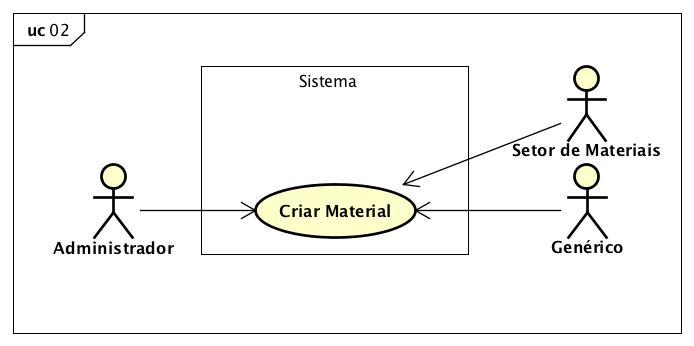
\includegraphics[width=10cm]{Imagens/UC_CriarMaterial.jpg}
	    \captionof{figure}{Diagrama do Caso de Uso Criar Material}
		\label{fig:uc_criar_material}
	\end{minipage} \\

	\begin{enumerate}[label=, leftmargin=0cm]
		\item \textbf{Atores} \\
		Administrador, Setor de Materiais e Genérico.
		\item \textbf{Precondições}
			\begin{enumerate}[label=\arabic*.]
				\item Existir oferta cadastrada com módulo e disciplina.
				\item Existir artefato de aula ou prova relacionado com a oferta.
				\item Existir um fluxo associado ao artefato.
				\item Usuários responsáveis pelas etapas do fluxo estarem logados no sistema.
			\end{enumerate}
		\item \textbf{Fluxo Básico}
			\begin{enumerate}[label=\arabic*.]
				\item Usuário solicita visualização da oferta.
				\item Sistema exibe dados da oferta com todos os artefatos (aula ou prova).
				\item Usuário seleciona artefato que deseja dar início ao processo de criação do material.
				\item Sistema exibe formulário de criação do material com campos para carregamento do arquivo, mensagem e possíveis próximas etapas para as quais esse material pode seguir.
				\item Usuário preenche o formulário, carrega o arquivo e define qual o próximo passo do fluxo.
				\item Sistema recebe os dados, informa ao usuário que o material foi submetido.
				\item Sistema notifica responsáveis pela etapa atual do material e aguarda ação.
				\item Usuário responsável pela etapa atual solicita visualização do material.
				\item Sistema exibe informações do material atual permitindo que o usuário baixe o arquivo.
				\item Usuário solicita criação de nova versão do material atual.
				\item Sistema mostra formulário de criação de nova versão do material atual com campos para carregamento do arquivo, mensagem e possíveis próximas etapas para as quais esse material pode seguir.
				\item Usuário preenche o formulário, carrega o arquivo e define qual o próximo passo do fluxo.
				\item Volta ao passo 6 e repete até que o material chegue à etapa final do fluxo.
				\item Sistema sinaliza que o fluxo do artefato foi completado e que o material está pronto.
			\end{enumerate}
		\item \textbf{Fluxo Alternativo A}
			\begin{enumerate}[label=\arabic*.]
				\item Ao fim do passo 2 do Fluxo básico, um usuário com papel de Administrador decide interver no fluxo e move o material para alguma etapa que não é necessariamente uma das disponíveis a partir da etapa atual.
				\item O fluxo retorna ao passo 13 do Fluxo Básico.
			\end{enumerate}
		\item \textbf{Pós-condições}
			\begin{enumerate}[label=\arabic*.]
				\item O estado de feito é atribuído ao artefato do material.
				\item Há um material pronto e disponível.
			\end{enumerate}
	\end{enumerate}
	 
\end{enumerate}


\section{Projeto de Interface}

Baseando-se nos requisitos elicitados, o projeto de interface foi realizado e os protótipos que serão apresentados a seguir, apesar de se tratarem de \textit{wireframes}, já trazem uma preocupação com a intuitividade e usabilidade do sistema.

O primeiro \textit{wireframe} (Figura \hyperref[fig:pi_tela_inicial]{\ref{fig:pi_tela_inicial}}) demonstra a tela inicial, que deve ser apresentada logo após o login do usuário. Nela, estão organizados alguns elementos como um espaço para alertas de materiais com o prazo emergencial, outro para últimas mensagens recebidas e os fluxos de trabalho ativos. Nesse último, cada bloco representa um fluxo de material cujo produto está na fase que o usuário atual é responsável por contribuir.

\vspace{5mm}
\begin{minipage}[c]{\textwidth}
    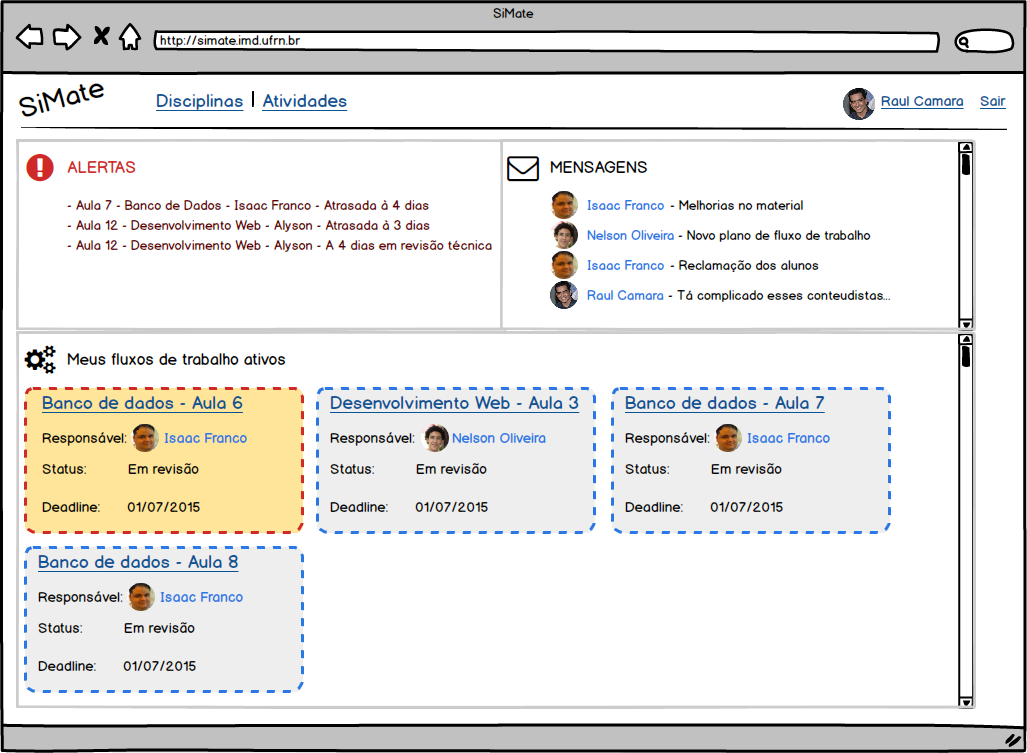
\includegraphics[width=15cm]{Imagens/SiMateTelas/Index.png}
    \captionof{figure}{Tela Inicial}
	\label{fig:pi_tela_inicial}
\end{minipage} \\

Através da barra de navegação do sistema, é possível visualizar as ofertas (representada por disciplinas) do usuário. Essa visualização é apresentada através da grade da Figura \hyperref[fig:pi_grade_disciplinas]{\ref{fig:pi_grade_disciplinas}}.

\vspace{5mm}
\begin{minipage}[c]{\textwidth}
    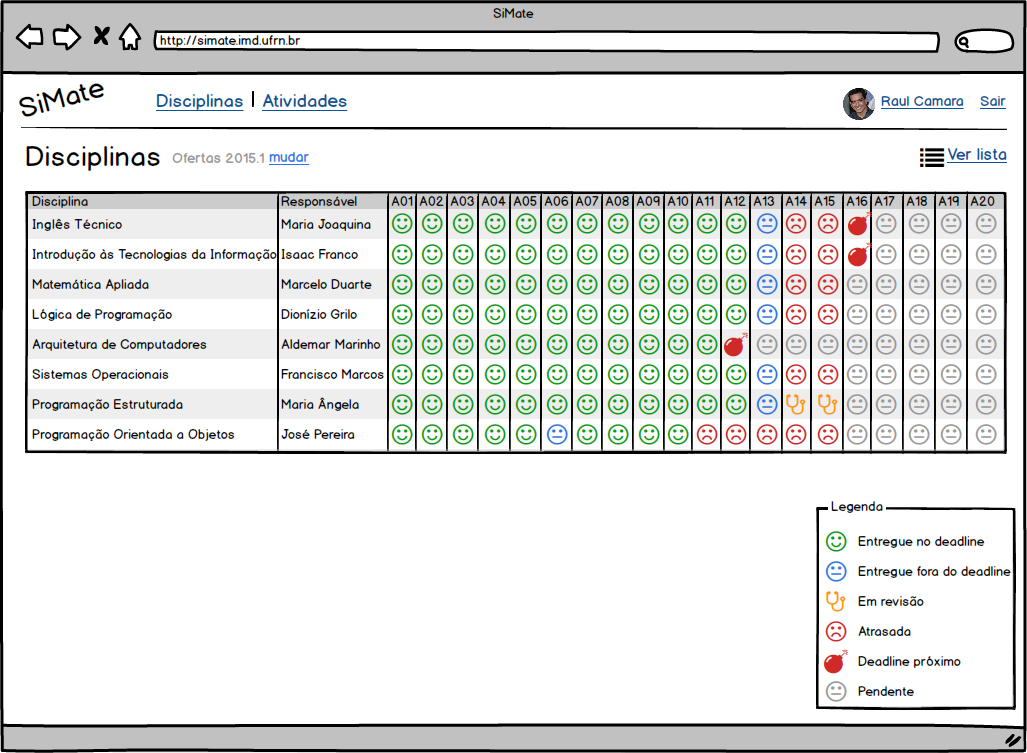
\includegraphics[width=15cm]{Imagens/SiMateTelas/GradeDisciplinas.png}
    \captionof{figure}{Tela de Listagem das Ofertas}
	\label{fig:pi_grade_disciplinas}
\end{minipage} \\

É possível notar que a grade de disciplinas possui uma coluna para responsável, esse é o usuário/equipe que deve dar início ao fluxo de criação do material, e colunas para os artefatos de aulas e provas. Cada artefato possui um estado que pode ser entendido através da legenda no canto inferior direito.

Na próxima tela (Figura \hyperref[fig:pi_artefato_detalhe]{\ref{fig:pi_artefato_detalhe}})), o fluxo do material é mostrado com os detalhes do artefato. 

\vspace{5mm}
\begin{minipage}[c]{\textwidth}
    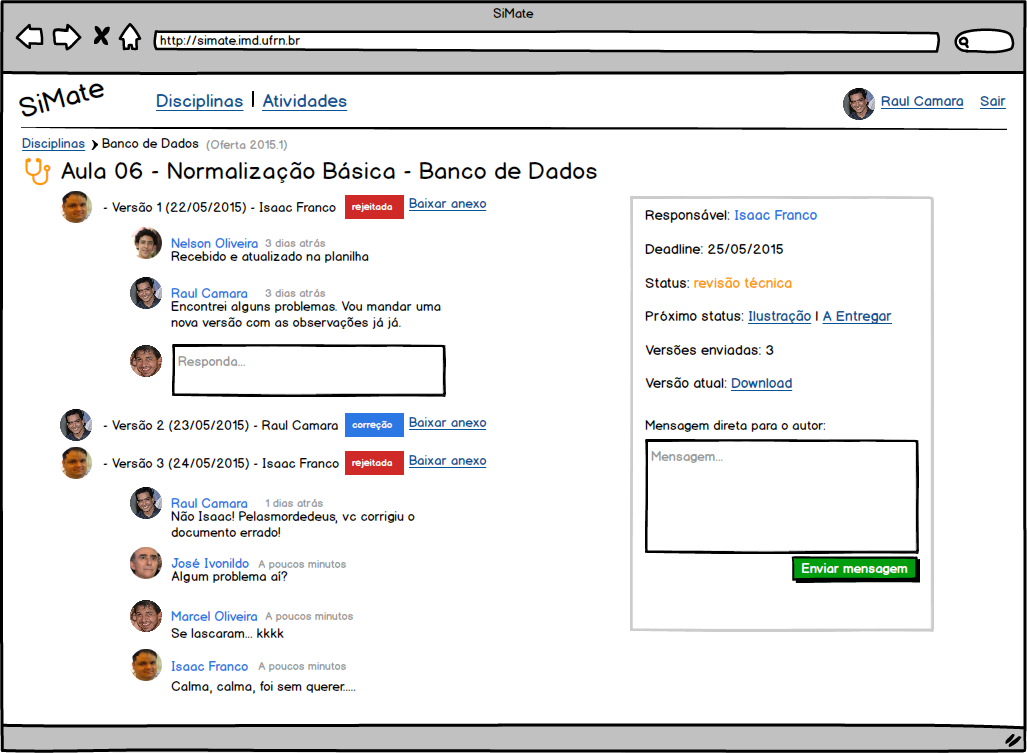
\includegraphics[width=15cm]{Imagens/SiMateTelas/ArtefatoDetalhe.png}
    \captionof{figure}{Tela de Detalhe do Artefato}
	\label{fig:pi_artefato_detalhe}
\end{minipage} \\

Cada versão do material na tela acima registra uma contribuição dentro do fluxo, uma passagem de etapa/passo. É nessa tela que a gerência do setor de materiais poderá entender de forma fácil e prática como anda o processo, podendo assim baixar todas as versões do produto, analisá-las e interagir com os envolvidos através de comentários. Caso seja necessário que o usuário envie uma nova revisão do material, é possível fazê-lo através do formulário presente no lado direito da tela e este será adicionado ao fim da listagem de versões como esperado.

\section{Arquitetura}

A arquitetura de implementação do projeto se baseia na usada pelo núcleo de desenvolvimento do Instituto Metrópole Digital e pode ser visualizada na figura abaixo.

\vspace{5mm}
\begin{minipage}[c]{\textwidth}
	\centering
    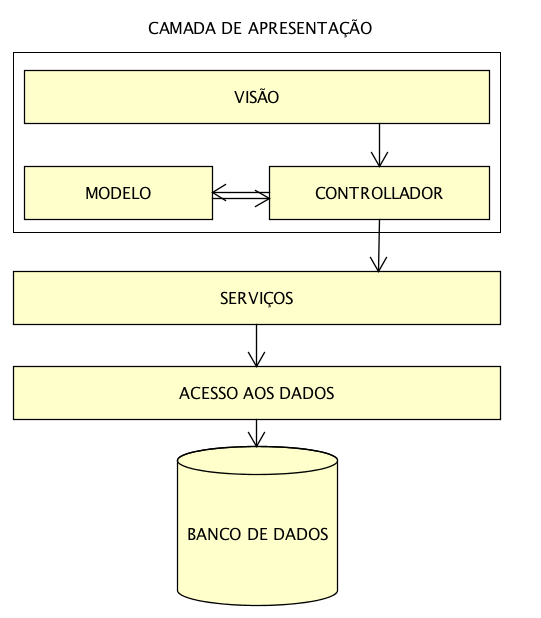
\includegraphics[width=10cm]{Imagens/Arquitetura.png}
    \captionof{figure}{Arquitetura Simplificada do SiMate}
	\label{fig:arq}
\end{minipage} \\

Na Figura \hyperref[fig:arq]{\ref{fig:arq}}, o primeira caixa representa a camada de apresentação no padrão MVC (Modelo - Visão - Controlador) que é um padrão de arquitetura de software onde a Visão representa as telas de interação e as saídas de dados, o modelo representa as regras de negócio e o controlador é o mediador que recebe as entradas através da visão e os converte em comandos gerando ou não uma saída pro usuário. Após isso temos a camada de serviços que oferece as ações disponíveis para manipulação de dados, ações essas que são executadas na camada de acesso aos dados.

	
	% Capitulo 3: Terceiro capítulo (arquivo Includes/Cronograma.tex)
	%% SiMate

\chapter{Cronograma}
		
	% Consideracoes finais
	%\include{Capitulos/Consideracoes}
	
	% Bibliografia (arquivo Capitulos/Referencias.bib)
	%\bibliography{Capitulos/Referencias}
	%\bibliographystyle{abnt-alf}
	
	% Apêndice A (arquivo Includes/ApendiceA)
	%\include{Capitulos/ApendiceA}
	
	% Anexo A (arquivo Includes/AnexoA)
	%\include{Capitulos/AnexoA}
	
	% Página em branco
	\newpage

\end{document}